\scanpage{18}
\margin{\handwritten{\unsure{1.9.3|1.93|1.9.5}, \unsure{1.27|1.23}, 2.9 à reporter au \unsure{n\textsuperscript{o} 3}\\\unsure{3.1}\ \unsure{?}}}

\(\mathbb{S}\)GA 4 VI

\uline{Sommaire}
\margin{\handwritten{\uline{\unsure{pp|pr}}}}

1. Conditions de finitude pour les objets et flêches d'un topos.\margin{\handwritten{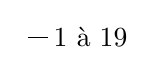
\begin{tikzpicture}[baseline=0,x=.45cm,y=.45cm]\draw (-.7,.12)--(-.15,.12);\node[anchor=west,inner sep=0pt] at (0,.12) {1 à 19};\end{tikzpicture}}}

2. Conditions de finitude pour un topos.\margin{\handwritten{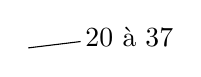
\begin{tikzpicture}[baseline=0,x=.45cm,y=.45cm]\draw (-1.6,-.18)--(-.12,0);\node[anchor=west,inner sep=0pt] at (0,.12) {20 à 37};\end{tikzpicture}}}

3. Conditions de finitude pour un morphisme de topos. \deleted{\handwritten{Cas des \unsure{topos} \unsure{inductifs|induits}}}\margin{\handwritten{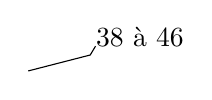
\begin{tikzpicture}[baseline=0,x=.45cm,y=.45cm]\draw (-1.9,-.5)--(-.15,-.05)--(0,.2);\node[anchor=west,inner sep=0pt] at (0,.45) {38 à 46};\end{tikzpicture}}}

\deleted{4. Constructibilité.}\inserted{\handwritten{4. Conditions de finitude pour un topos \inserted{obtenu par} recollement.}}\margin{\handwritten{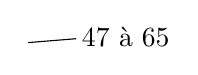
\begin{tikzpicture}[baseline=0,x=.45cm,y=.45cm]\draw (-1.5,-.03)--(-.15,.08);\node[anchor=west,inner sep=0pt] at (0,.12) {47 à 65};\end{tikzpicture}}}
% The pencil divider is immediately beneath the original and replacement item 4.
\noindent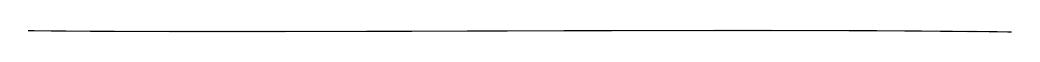
\begin{tikzpicture}[x=\linewidth,y=.4cm]\draw (-.07,0)..controls (.2,-.08) and (.7,.08)..(.96,-.04);\end{tikzpicture}
% The relocation curve remains in the LEFT margin, with its question mark;
% its lower end is beside the circled replacement 5 and its arrowhead points
% to the divider after item 4. The drawing preserves the source's relative geometry.
\reversemarginpar
\margin{\handwritten{\begin{tikzpicture}[x=.55cm,y=.55cm]
\draw[->] (2,-6.5)..controls (-1,-4.6) and (-1,-3.2)..(2,0);
\node at (.05,-1.8) {?};
\end{tikzpicture}}}
\normalmarginpar

\deleted{5}\handwritten{6}. Catégories fibrées et $\underset{\handwritten{\longrightarrow}}{\mathrm{Lim}}$ (rappels).

\deleted{6}\handwritten{7}. Sites et topos fibrés.

\reversemarginpar
\margin{\handwritten{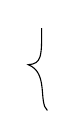
\begin{tikzpicture}[x=.45cm,y=.45cm]
\draw (1,0)..controls (1,-.8) and (1,-1.0)..(.62,-1.03)
 ..controls (1.2,-1.25) and (.9,-2.1)..(1.16,-2.32);
\end{tikzpicture}}}
\normalmarginpar
\deleted{7}\handwritten{8}. Limites projectives de topos.

\deleted{8}\handwritten{\unsure{8|9}}. Cas des limites projectives filtrantes de topos cohérents par morphismes de transition cohérents: théorèmes de passage à la limite pour la cohomologie.

\noindent\begin{tikzpicture}[baseline=(n.base)]\node[draw,ellipse,inner sep=3pt] (n) {\deleted{9}\handwritten{5}.};\end{tikzpicture} Cohomologie d'une limite inductive de fais\unsure{\deleted{x}c|\deleted{c}x}eaux sur un topos cohérent
% The right edge cuts immediately after the t of cohérent; no full stop is visible.

\reversemarginpar
\margin{\handwritten{\begin{tikzpicture}[x=.25cm,y=.25cm]\draw[line width=2pt] (0,0)--(.04,-.55);\end{tikzpicture}}}
\normalmarginpar
\handwritten{10. Appendice (par P. Deligne). \deleted{Existence de points \unsure{d'}}\unsure{Un} topos cohérent \unsure{a} \inserted{suffisamment de points}.}

\deleted{NB \(\mathbb{B}\)ien sûr \deleted{\unsure{9}}\handwritten{8} serait interchangeable avec le bloc \deleted{5}\handwritten{4} à \deleted{8}\handwritten{9}. Mais il me semble plus naturel de mettre dans deux numéros consécuti\unsure{\deleted{s}f|\deleted{f}s}s les deux facettes d\unsure{\deleted{y}u|\deleted{g}u|\deleted{u}y|\deleted{u}g} \unsure{\deleted{b}p|\deleted{p}b}assage à la limite en cohomologie. Bien sûr, le numéro \deleted{9}\handwritten{8} sera réduit à une ou deux pages, le sorite des conditions de finitude étant déjà fait.}

\deleted{Le n\textsuperscript{\uline{o}} 4 contiendra le sorite des groupes constructibles (au sens groupes finis ou non), des faisceaux de torsion, des notions de constructibilité pour les Modules et complexes de Modules, - y compris les faits spéciaux dans le cas localement noethérien. Je pense que je le rédigerai mais ne le garantis pas. On peut \deleted{\unsure{à la rigue|à la rigueur}} laisser t\deleted{\unsure{l}}\handwritten{o}mber le n\textsuperscript{\uline{o}}4, ce sera alors moins beau bien sûr ...:}

\deleted{La rédaction qui suit des n\textsuperscript{\uline{o}}s 1 à 3 est àomplète, à cela près que je compte y ajouter encore quelques exemples (en particulier un topos localement algébrique non algébrique\inserted{\handwritten{)}}\unsure{,|.} \deleted{un morphisme non cohérent de topos cohérents).}}
\reversemarginpar
\margin{\handwritten{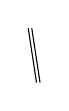
\begin{tikzpicture}[x=.3cm,y=.3cm]\draw (0,0)--(.35,-2.3);\draw (.15,0)--(.5,-2.3);\end{tikzpicture}}}
\normalmarginpar
\inserted{\handwritten{et un topos ayant une famille génératrice formée d'objet\unsure{s} cohérents, qui n'est pas localement algébrique}}
% archive sheet number: 17
